\documentclass[1p]{elsarticle_modified}
%\bibliographystyle{elsarticle-num}

%\usepackage[colorlinks]{hyperref}
%\usepackage{abbrmath_seonhwa} %\Abb, \Ascr, \Acal ,\Abf, \Afrak
\usepackage{amsfonts}
\usepackage{amssymb}
\usepackage{amsmath}
\usepackage{amsthm}
\usepackage{scalefnt}
\usepackage{amsbsy}
\usepackage{kotex}
\usepackage{caption}
\usepackage{subfig}
\usepackage{color}
\usepackage{graphicx}
\usepackage{xcolor} %% white, black, red, green, blue, cyan, magenta, yellow
\usepackage{float}
\usepackage{setspace}
\usepackage{hyperref}

\usepackage{tikz}
\usetikzlibrary{arrows}

\usepackage{multirow}
\usepackage{array} % fixed length table
\usepackage{hhline}

%%%%%%%%%%%%%%%%%%%%%
\makeatletter
\renewcommand*\env@matrix[1][\arraystretch]{%
	\edef\arraystretch{#1}%
	\hskip -\arraycolsep
	\let\@ifnextchar\new@ifnextchar
	\array{*\c@MaxMatrixCols c}}
\makeatother %https://tex.stackexchange.com/questions/14071/how-can-i-increase-the-line-spacing-in-a-matrix
%%%%%%%%%%%%%%%

\usepackage[normalem]{ulem}

\newcommand{\msout}[1]{\ifmmode\text{\sout{\ensuremath{#1}}}\else\sout{#1}\fi}
%SOURCE: \msout is \stkout macro in https://tex.stackexchange.com/questions/20609/strikeout-in-math-mode

\newcommand{\cancel}[1]{
	\ifmmode
	{\color{red}\msout{#1}}
	\else
	{\color{red}\sout{#1}}
	\fi
}

\newcommand{\add}[1]{
	{\color{blue}\uwave{#1}}
}

\newcommand{\replace}[2]{
	\ifmmode
	{\color{red}\msout{#1}}{\color{blue}\uwave{#2}}
	\else
	{\color{red}\sout{#1}}{\color{blue}\uwave{#2}}
	\fi
}

\newcommand{\Sol}{\mathcal{S}} %segment
\newcommand{\D}{D} %diagram
\newcommand{\A}{\mathcal{A}} %arc


%%%%%%%%%%%%%%%%%%%%%%%%%%%%%5 test

\def\sl{\operatorname{\textup{SL}}(2,\Cbb)}
\def\psl{\operatorname{\textup{PSL}}(2,\Cbb)}
\def\quan{\mkern 1mu \triangleright \mkern 1mu}

\theoremstyle{definition}
\newtheorem{thm}{Theorem}[section]
\newtheorem{prop}[thm]{Proposition}
\newtheorem{lem}[thm]{Lemma}
\newtheorem{ques}[thm]{Question}
\newtheorem{cor}[thm]{Corollary}
\newtheorem{defn}[thm]{Definition}
\newtheorem{exam}[thm]{Example}
\newtheorem{rmk}[thm]{Remark}
\newtheorem{alg}[thm]{Algorithm}

\newcommand{\I}{\sqrt{-1}}
\begin{document}

%\begin{frontmatter}
%
%\title{Boundary parabolic representations of knots up to 8 crossings}
%
%%% Group authors per affiliation:
%\author{Yunhi Cho} 
%\address{Department of Mathematics, University of Seoul, Seoul, Korea}
%\ead{yhcho@uos.ac.kr}
%
%
%\author{Seonhwa Kim} %\fnref{s_kim}}
%\address{Center for Geometry and Physics, Institute for Basic Science, Pohang, 37673, Korea}
%\ead{ryeona17@ibs.re.kr}
%
%\author{Hyuk Kim}
%\address{Department of Mathematical Sciences, Seoul National University, Seoul 08826, Korea}
%\ead{hyukkim@snu.ac.kr}
%
%\author{Seokbeom Yoon}
%\address{Department of Mathematical Sciences, Seoul National University, Seoul, 08826,  Korea}
%\ead{sbyoon15@snu.ac.kr}
%
%\begin{abstract}
%We find all boundary parabolic representation of knots up to 8 crossings.
%
%\end{abstract}
%\begin{keyword}
%    \MSC[2010] 57M25 
%\end{keyword}
%
%\end{frontmatter}

%\linenumbers
%\tableofcontents
%
\newcommand\colored[1]{\textcolor{white}{\rule[-0.35ex]{0.8em}{1.4ex}}\kern-0.8em\color{red} #1}%
%\newcommand\colored[1]{\textcolor{white}{ #1}\kern-2.17ex	\textcolor{white}{ #1}\kern-1.81ex	\textcolor{white}{ #1}\kern-2.15ex\color{red}#1	}

{\Large $\underline{12n_{0589}~(K12n_{0589})}$}

\setlength{\tabcolsep}{10pt}
\renewcommand{\arraystretch}{1.6}
\vspace{1cm}\begin{tabular}{m{100pt}>{\centering\arraybackslash}m{274pt}}
\multirow{5}{120pt}{
	\centering
	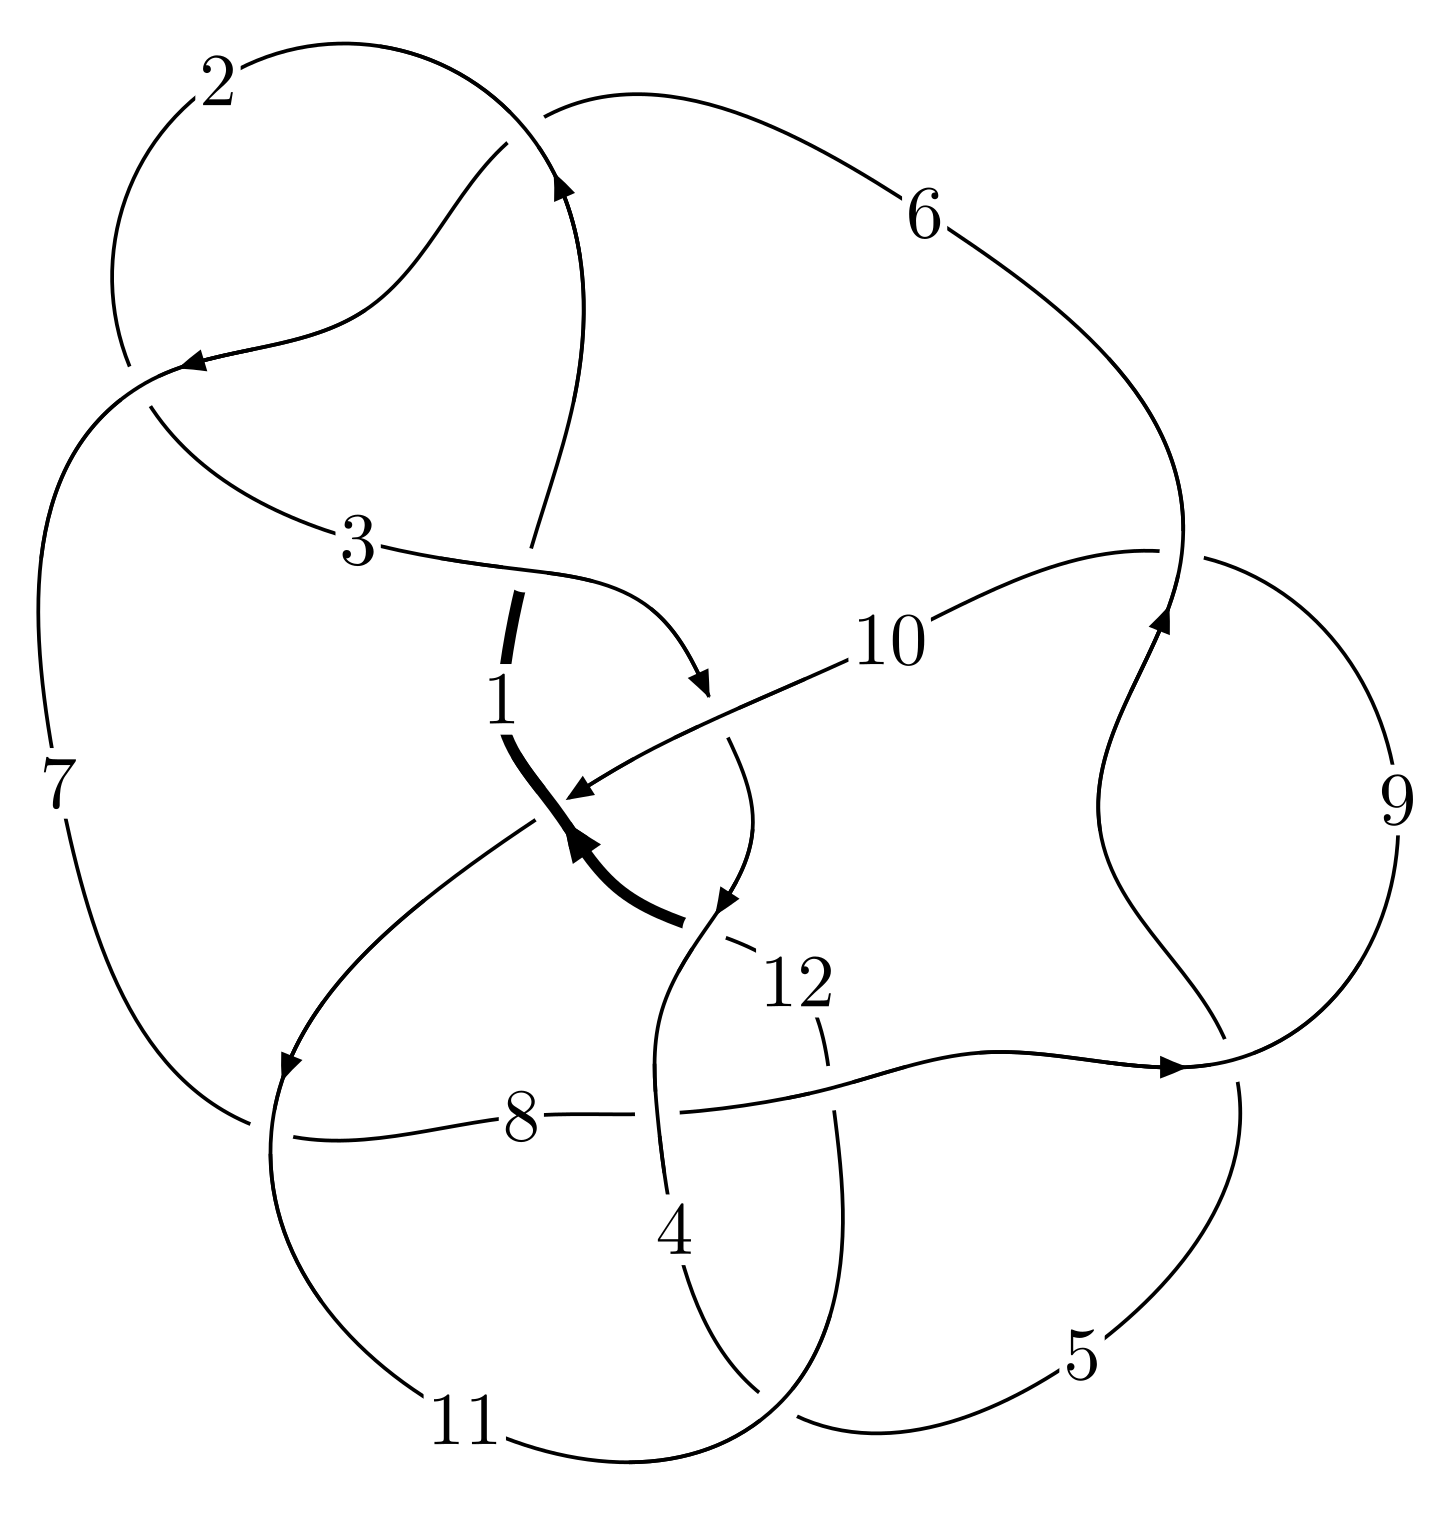
\includegraphics[width=112pt]{../../../GIT/diagram.site/Diagrams/png/2678_12n_0589.png}\\
\ \ \ A knot diagram\footnotemark}&
\allowdisplaybreaks
\textbf{Linearized knot diagam} \\
\cline{2-2}
 &
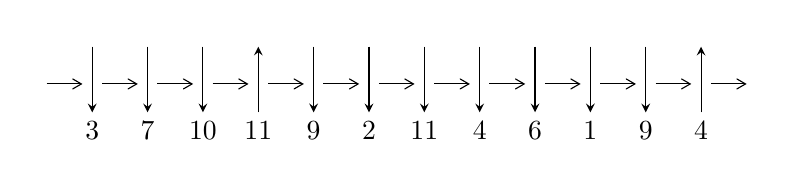
\begin{tikzpicture}[x=20pt, y=17pt]
	% nodes
	\node (C0) at (0, 0) {};
	\node (C1) at (1, 0) {};
	\node (C1U) at (1, +1) {};
	\node (C1D) at (1, -1) {3};

	\node (C2) at (2, 0) {};
	\node (C2U) at (2, +1) {};
	\node (C2D) at (2, -1) {7};

	\node (C3) at (3, 0) {};
	\node (C3U) at (3, +1) {};
	\node (C3D) at (3, -1) {10};

	\node (C4) at (4, 0) {};
	\node (C4U) at (4, +1) {};
	\node (C4D) at (4, -1) {11};

	\node (C5) at (5, 0) {};
	\node (C5U) at (5, +1) {};
	\node (C5D) at (5, -1) {9};

	\node (C6) at (6, 0) {};
	\node (C6U) at (6, +1) {};
	\node (C6D) at (6, -1) {2};

	\node (C7) at (7, 0) {};
	\node (C7U) at (7, +1) {};
	\node (C7D) at (7, -1) {11};

	\node (C8) at (8, 0) {};
	\node (C8U) at (8, +1) {};
	\node (C8D) at (8, -1) {4};

	\node (C9) at (9, 0) {};
	\node (C9U) at (9, +1) {};
	\node (C9D) at (9, -1) {6};

	\node (C10) at (10, 0) {};
	\node (C10U) at (10, +1) {};
	\node (C10D) at (10, -1) {1};

	\node (C11) at (11, 0) {};
	\node (C11U) at (11, +1) {};
	\node (C11D) at (11, -1) {9};

	\node (C12) at (12, 0) {};
	\node (C12U) at (12, +1) {};
	\node (C12D) at (12, -1) {4};
	\node (C13) at (13, 0) {};

	% arrows
	\draw[->,>={angle 60}]
	(C0) edge (C1) (C1) edge (C2) (C2) edge (C3) (C3) edge (C4) (C4) edge (C5) (C5) edge (C6) (C6) edge (C7) (C7) edge (C8) (C8) edge (C9) (C9) edge (C10) (C10) edge (C11) (C11) edge (C12) (C12) edge (C13) ;	\draw[->,>=stealth]
	(C1U) edge (C1D) (C2U) edge (C2D) (C3U) edge (C3D) (C4D) edge (C4U) (C5U) edge (C5D) (C6U) edge (C6D) (C7U) edge (C7D) (C8U) edge (C8D) (C9U) edge (C9D) (C10U) edge (C10D) (C11U) edge (C11D) (C12D) edge (C12U) ;
	\end{tikzpicture} \\
\hhline{~~} \\& 
\textbf{Solving Sequence} \\ \cline{2-2} 
 &
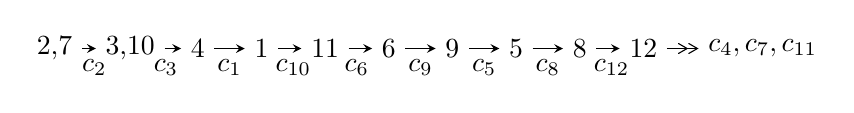
\begin{tikzpicture}[x=23pt, y=7pt]
	% node
	\node (A0) at (-1/8, 0) {2,7};
	\node (A1) at (17/16, 0) {3,10};
	\node (A2) at (17/8, 0) {4};
	\node (A3) at (25/8, 0) {1};
	\node (A4) at (33/8, 0) {11};
	\node (A5) at (41/8, 0) {6};
	\node (A6) at (49/8, 0) {9};
	\node (A7) at (57/8, 0) {5};
	\node (A8) at (65/8, 0) {8};
	\node (A9) at (73/8, 0) {12};
	\node (C1) at (1/2, -1) {$c_{2}$};
	\node (C2) at (13/8, -1) {$c_{3}$};
	\node (C3) at (21/8, -1) {$c_{1}$};
	\node (C4) at (29/8, -1) {$c_{10}$};
	\node (C5) at (37/8, -1) {$c_{6}$};
	\node (C6) at (45/8, -1) {$c_{9}$};
	\node (C7) at (53/8, -1) {$c_{5}$};
	\node (C8) at (61/8, -1) {$c_{8}$};
	\node (C9) at (69/8, -1) {$c_{12}$};
	\node (A10) at (11, 0) {$c_{4},c_{7},c_{11}$};

	% edge
	\draw[->,>=stealth]	
	(A0) edge (A1) (A1) edge (A2) (A2) edge (A3) (A3) edge (A4) (A4) edge (A5) (A5) edge (A6) (A6) edge (A7) (A7) edge (A8) (A8) edge (A9) ;
	\draw[->>,>={angle 60}]	
	(A9) edge (A10);
\end{tikzpicture} \\ 

\end{tabular} \\

\footnotetext{
The image of knot diagram is generated by the software ``\textbf{Draw programme}" developed by Andrew Bartholomew(\url{http://www.layer8.co.uk/maths/draw/index.htm\#Running-draw}), where we modified some parts for our purpose(\url{https://github.com/CATsTAILs/LinksPainter}).
}\phantom \\ \newline 
\centering \textbf{Ideals for irreducible components\footnotemark of $X_{\text{par}}$} 
 
\begin{align*}
I^u_{1}&=\langle 
2.15027\times10^{88} u^{78}+3.02788\times10^{88} u^{77}+\cdots+2.41970\times10^{87} b-3.63043\times10^{89},\\
\phantom{I^u_{1}}&\phantom{= \langle  }2.91093\times10^{89} u^{78}+3.67504\times10^{89} u^{77}+\cdots+1.57280\times10^{88} a-4.88443\times10^{90},\;u^{79}+2 u^{78}+\cdots- u-13\rangle \\
I^u_{2}&=\langle 
-696 u^{22}+792 u^{21}+\cdots+302 b-1145,\;-655 u^{22}+334 u^{21}+\cdots+151 a-725,\\
\phantom{I^u_{2}}&\phantom{= \langle  }u^{23}- u^{22}+\cdots+3 u-1\rangle \\
\\
\end{align*}
\raggedright * 2 irreducible components of $\dim_{\mathbb{C}}=0$, with total 102 representations.\\
\footnotetext{All coefficients of polynomials are rational numbers. But the coefficients are sometimes approximated in decimal forms when there is not enough margin.}
\newpage
\renewcommand{\arraystretch}{1}
\centering \section*{I. $I^u_{1}= \langle 2.15\times10^{88} u^{78}+3.03\times10^{88} u^{77}+\cdots+2.42\times10^{87} b-3.63\times10^{89},\;2.91\times10^{89} u^{78}+3.68\times10^{89} u^{77}+\cdots+1.57\times10^{88} a-4.88\times10^{90},\;u^{79}+2 u^{78}+\cdots- u-13 \rangle$}
\flushleft \textbf{(i) Arc colorings}\\
\begin{tabular}{m{7pt} m{180pt} m{7pt} m{180pt} }
\flushright $a_{2}=$&$\begin{pmatrix}1\\0\end{pmatrix}$ \\
\flushright $a_{7}=$&$\begin{pmatrix}0\\u\end{pmatrix}$ \\
\flushright $a_{3}=$&$\begin{pmatrix}1\\u^2\end{pmatrix}$ \\
\flushright $a_{10}=$&$\begin{pmatrix}-18.5079 u^{78}-23.3662 u^{77}+\cdots-380.443 u+310.556\\-8.88654 u^{78}-12.5135 u^{77}+\cdots-158.149 u+150.037\end{pmatrix}$ \\
\flushright $a_{4}=$&$\begin{pmatrix}-1.64242 u^{78}-5.44213 u^{77}+\cdots-146.208 u+80.9180\\-3.47633 u^{78}-9.10119 u^{77}+\cdots-197.562 u+125.360\end{pmatrix}$ \\
\flushright $a_{1}=$&$\begin{pmatrix}- u^2+1\\- u^4\end{pmatrix}$ \\
\flushright $a_{11}=$&$\begin{pmatrix}-12.0911 u^{78}-16.6948 u^{77}+\cdots-315.397 u+227.813\\-5.48169 u^{78}-10.3261 u^{77}+\cdots-177.652 u+129.008\end{pmatrix}$ \\
\flushright $a_{6}=$&$\begin{pmatrix}u\\u\end{pmatrix}$ \\
\flushright $a_{9}=$&$\begin{pmatrix}-11.3809 u^{78}-15.4740 u^{77}+\cdots-263.755 u+201.485\\-1.75952 u^{78}-4.62127 u^{77}+\cdots-41.4612 u+40.9657\end{pmatrix}$ \\
\flushright $a_{5}=$&$\begin{pmatrix}-10.4501 u^{78}-16.1921 u^{77}+\cdots-418.113 u+259.056\\3.24517 u^{78}+1.05048 u^{77}+\cdots-92.9910 u+13.4345\end{pmatrix}$ \\
\flushright $a_{8}=$&$\begin{pmatrix}25.1053 u^{78}+33.6322 u^{77}+\cdots+612.317 u-456.608\\22.1871 u^{78}+27.8524 u^{77}+\cdots+413.354 u-348.620\end{pmatrix}$ \\
\flushright $a_{12}=$&$\begin{pmatrix}-11.2839 u^{78}-11.8219 u^{77}+\cdots-210.236 u+164.805\\-9.08712 u^{78}-6.33482 u^{77}+\cdots-59.2341 u+78.4719\end{pmatrix}$\\&\end{tabular}
\flushleft \textbf{(ii) Obstruction class $= -1$}\\~\\
\flushleft \textbf{(iii) Cusp Shapes $= 25.2924 u^{78}+32.9982 u^{77}+\cdots+728.389 u-509.327$}\\~\\
\newpage\renewcommand{\arraystretch}{1}
\flushleft \textbf{(iv) u-Polynomials at the component}\newline \\
\begin{tabular}{m{50pt}|m{274pt}}
Crossings & \hspace{64pt}u-Polynomials at each crossing \\
\hline $$\begin{aligned}c_{1}\end{aligned}$$&$\begin{aligned}
&u^{79}+36 u^{78}+\cdots+3641 u+169
\end{aligned}$\\
\hline $$\begin{aligned}c_{2},c_{6}\end{aligned}$$&$\begin{aligned}
&u^{79}-2 u^{78}+\cdots- u+13
\end{aligned}$\\
\hline $$\begin{aligned}c_{3}\end{aligned}$$&$\begin{aligned}
&u^{79}+2 u^{78}+\cdots-49 u+29
\end{aligned}$\\
\hline $$\begin{aligned}c_{4}\end{aligned}$$&$\begin{aligned}
&u^{79}-2 u^{78}+\cdots+107183 u+13051
\end{aligned}$\\
\hline $$\begin{aligned}c_{5},c_{9}\end{aligned}$$&$\begin{aligned}
&u^{79}+3 u^{78}+\cdots+12688 u+2456
\end{aligned}$\\
\hline $$\begin{aligned}c_{7}\end{aligned}$$&$\begin{aligned}
&u^{79}-3 u^{78}+\cdots-2215654 u+836419
\end{aligned}$\\
\hline $$\begin{aligned}c_{8}\end{aligned}$$&$\begin{aligned}
&u^{79}- u^{78}+\cdots+77402 u+12427
\end{aligned}$\\
\hline $$\begin{aligned}c_{10}\end{aligned}$$&$\begin{aligned}
&u^{79}-9 u^{78}+\cdots+106 u+47
\end{aligned}$\\
\hline $$\begin{aligned}c_{11}\end{aligned}$$&$\begin{aligned}
&u^{79}+2 u^{78}+\cdots+84233 u+4289
\end{aligned}$\\
\hline $$\begin{aligned}c_{12}\end{aligned}$$&$\begin{aligned}
&u^{79}+12 u^{78}+\cdots+280 u+8
\end{aligned}$\\
\hline
\end{tabular}\\~\\
\newpage\renewcommand{\arraystretch}{1}
\flushleft \textbf{(v) Riley Polynomials at the component}\newline \\
\begin{tabular}{m{50pt}|m{274pt}}
Crossings & \hspace{64pt}Riley Polynomials at each crossing \\
\hline $$\begin{aligned}c_{1}\end{aligned}$$&$\begin{aligned}
&y^{79}+24 y^{78}+\cdots-134679 y-28561
\end{aligned}$\\
\hline $$\begin{aligned}c_{2},c_{6}\end{aligned}$$&$\begin{aligned}
&y^{79}-36 y^{78}+\cdots+3641 y-169
\end{aligned}$\\
\hline $$\begin{aligned}c_{3}\end{aligned}$$&$\begin{aligned}
&y^{79}+2 y^{78}+\cdots-1079 y-841
\end{aligned}$\\
\hline $$\begin{aligned}c_{4}\end{aligned}$$&$\begin{aligned}
&y^{79}-90 y^{78}+\cdots+7988152207 y-170328601
\end{aligned}$\\
\hline $$\begin{aligned}c_{5},c_{9}\end{aligned}$$&$\begin{aligned}
&y^{79}-37 y^{78}+\cdots+161614080 y-6031936
\end{aligned}$\\
\hline $$\begin{aligned}c_{7}\end{aligned}$$&$\begin{aligned}
&y^{79}+41 y^{78}+\cdots-12372523428214 y-699596743561
\end{aligned}$\\
\hline $$\begin{aligned}c_{8}\end{aligned}$$&$\begin{aligned}
&y^{79}+105 y^{78}+\cdots-6895853666 y-154430329
\end{aligned}$\\
\hline $$\begin{aligned}c_{10}\end{aligned}$$&$\begin{aligned}
&y^{79}+23 y^{78}+\cdots+385450 y-2209
\end{aligned}$\\
\hline $$\begin{aligned}c_{11}\end{aligned}$$&$\begin{aligned}
&y^{79}+84 y^{78}+\cdots-314032055 y-18395521
\end{aligned}$\\
\hline $$\begin{aligned}c_{12}\end{aligned}$$&$\begin{aligned}
&y^{79}-32 y^{78}+\cdots+3520 y-64
\end{aligned}$\\
\hline
\end{tabular}\\~\\
\newpage\flushleft \textbf{(vi) Complex Volumes and Cusp Shapes}
$$\begin{array}{c|c|c}  
\text{Solutions to }I^u_{1}& \I (\text{vol} + \sqrt{-1}CS) & \text{Cusp shape}\\
 \hline 
\begin{aligned}
u &= -0.940912 + 0.374623 I \\
a &= \phantom{-}1.04398 + 1.79768 I \\
b &= \phantom{-}1.77718 + 1.09794 I\end{aligned}
 & -3.10628 + 1.42293 I & \phantom{-0.000000 } 0 \\ \hline\begin{aligned}
u &= -0.940912 - 0.374623 I \\
a &= \phantom{-}1.04398 - 1.79768 I \\
b &= \phantom{-}1.77718 - 1.09794 I\end{aligned}
 & -3.10628 - 1.42293 I & \phantom{-0.000000 } 0 \\ \hline\begin{aligned}
u &= -0.907169 + 0.464698 I \\
a &= \phantom{-}1.56697 + 0.93171 I \\
b &= \phantom{-}0.718320 - 0.310140 I\end{aligned}
 & -2.40821 + 3.46296 I & \phantom{-0.000000 } 0 \\ \hline\begin{aligned}
u &= -0.907169 - 0.464698 I \\
a &= \phantom{-}1.56697 - 0.93171 I \\
b &= \phantom{-}0.718320 + 0.310140 I\end{aligned}
 & -2.40821 - 3.46296 I & \phantom{-0.000000 } 0 \\ \hline\begin{aligned}
u &= \phantom{-}0.611431 + 0.761311 I \\
a &= -0.210481 + 1.145050 I \\
b &= -1.68554 + 0.65090 I\end{aligned}
 & \phantom{-}9.90785 + 3.17209 I & \phantom{-0.000000 } 0 \\ \hline\begin{aligned}
u &= \phantom{-}0.611431 - 0.761311 I \\
a &= -0.210481 - 1.145050 I \\
b &= -1.68554 - 0.65090 I\end{aligned}
 & \phantom{-}9.90785 - 3.17209 I & \phantom{-0.000000 } 0 \\ \hline\begin{aligned}
u &= -0.362511 + 0.898774 I \\
a &= \phantom{-}0.549996 + 0.889051 I \\
b &= \phantom{-}0.831285 - 0.017175 I\end{aligned}
 & \phantom{-}0.89320 - 3.95862 I & \phantom{-0.000000 } 0 \\ \hline\begin{aligned}
u &= -0.362511 - 0.898774 I \\
a &= \phantom{-}0.549996 - 0.889051 I \\
b &= \phantom{-}0.831285 + 0.017175 I\end{aligned}
 & \phantom{-}0.89320 + 3.95862 I & \phantom{-0.000000 } 0 \\ \hline\begin{aligned}
u &= -0.857614 + 0.445269 I \\
a &= -0.015635 + 1.020300 I \\
b &= \phantom{-}1.60077 + 1.38290 I\end{aligned}
 & -2.20981 + 0.24877 I & \phantom{-0.000000 } 0 \\ \hline\begin{aligned}
u &= -0.857614 - 0.445269 I \\
a &= -0.015635 - 1.020300 I \\
b &= \phantom{-}1.60077 - 1.38290 I\end{aligned}
 & -2.20981 - 0.24877 I & \phantom{-0.000000 } 0\\
 \hline 
 \end{array}$$\newpage$$\begin{array}{c|c|c}  
\text{Solutions to }I^u_{1}& \I (\text{vol} + \sqrt{-1}CS) & \text{Cusp shape}\\
 \hline 
\begin{aligned}
u &= \phantom{-}0.941507 + 0.443174 I \\
a &= \phantom{-}0.17692 - 1.53807 I \\
b &= \phantom{-}0.964686 - 0.947975 I\end{aligned}
 & -2.31907 - 1.56521 I & \phantom{-0.000000 } 0 \\ \hline\begin{aligned}
u &= \phantom{-}0.941507 - 0.443174 I \\
a &= \phantom{-}0.17692 + 1.53807 I \\
b &= \phantom{-}0.964686 + 0.947975 I\end{aligned}
 & -2.31907 + 1.56521 I & \phantom{-0.000000 } 0 \\ \hline\begin{aligned}
u &= \phantom{-}0.467521 + 0.836388 I \\
a &= -1.24982 + 0.92072 I \\
b &= -0.870558 - 0.363496 I\end{aligned}
 & -0.94854 + 2.58619 I & \phantom{-0.000000 } 0 \\ \hline\begin{aligned}
u &= \phantom{-}0.467521 - 0.836388 I \\
a &= -1.24982 - 0.92072 I \\
b &= -0.870558 + 0.363496 I\end{aligned}
 & -0.94854 - 2.58619 I & \phantom{-0.000000 } 0 \\ \hline\begin{aligned}
u &= -0.882470 + 0.371777 I \\
a &= -1.09764 - 1.93772 I \\
b &= -1.59024 - 2.39194 I\end{aligned}
 & \phantom{-}4.16992 - 1.43305 I & \phantom{-0.000000 } 0 \\ \hline\begin{aligned}
u &= -0.882470 - 0.371777 I \\
a &= -1.09764 + 1.93772 I \\
b &= -1.59024 + 2.39194 I\end{aligned}
 & \phantom{-}4.16992 + 1.43305 I & \phantom{-0.000000 } 0 \\ \hline\begin{aligned}
u &= \phantom{-}1.020540 + 0.220943 I \\
a &= -0.877902 - 0.130605 I \\
b &= \phantom{-}0.274153 - 0.994301 I\end{aligned}
 & \phantom{-}0.64583 + 1.61580 I & \phantom{-0.000000 } 0 \\ \hline\begin{aligned}
u &= \phantom{-}1.020540 - 0.220943 I \\
a &= -0.877902 + 0.130605 I \\
b &= \phantom{-}0.274153 + 0.994301 I\end{aligned}
 & \phantom{-}0.64583 - 1.61580 I & \phantom{-0.000000 } 0 \\ \hline\begin{aligned}
u &= -0.471684 + 0.939721 I \\
a &= -1.06369 - 1.04214 I \\
b &= -1.211420 + 0.417868 I\end{aligned}
 & \phantom{-}7.30955 - 10.88550 I & \phantom{-0.000000 } 0 \\ \hline\begin{aligned}
u &= -0.471684 - 0.939721 I \\
a &= -1.06369 + 1.04214 I \\
b &= -1.211420 - 0.417868 I\end{aligned}
 & \phantom{-}7.30955 + 10.88550 I & \phantom{-0.000000 } 0\\
 \hline 
 \end{array}$$\newpage$$\begin{array}{c|c|c}  
\text{Solutions to }I^u_{1}& \I (\text{vol} + \sqrt{-1}CS) & \text{Cusp shape}\\
 \hline 
\begin{aligned}
u &= -0.627645 + 0.696624 I \\
a &= -0.521853 - 0.958627 I \\
b &= -1.092110 - 0.473148 I\end{aligned}
 & \phantom{-}2.90030 + 0.96581 I & \phantom{-0.000000 } 0 \\ \hline\begin{aligned}
u &= -0.627645 - 0.696624 I \\
a &= -0.521853 + 0.958627 I \\
b &= -1.092110 + 0.473148 I\end{aligned}
 & \phantom{-}2.90030 - 0.96581 I & \phantom{-0.000000 } 0 \\ \hline\begin{aligned}
u &= -1.057960 + 0.098937 I \\
a &= \phantom{-}0.378289 + 0.870614 I \\
b &= -0.607534 + 0.534343 I\end{aligned}
 & -4.85614 - 2.30083 I & \phantom{-0.000000 } 0 \\ \hline\begin{aligned}
u &= -1.057960 - 0.098937 I \\
a &= \phantom{-}0.378289 - 0.870614 I \\
b &= -0.607534 - 0.534343 I\end{aligned}
 & -4.85614 + 2.30083 I & \phantom{-0.000000 } 0 \\ \hline\begin{aligned}
u &= \phantom{-}0.273338 + 0.890041 I \\
a &= -0.037137 - 1.377140 I \\
b &= \phantom{-}0.452185 - 0.240610 I\end{aligned}
 & \phantom{-}7.98072 - 0.14474 I & \phantom{-0.000000 } 0 \\ \hline\begin{aligned}
u &= \phantom{-}0.273338 - 0.890041 I \\
a &= -0.037137 + 1.377140 I \\
b &= \phantom{-}0.452185 + 0.240610 I\end{aligned}
 & \phantom{-}7.98072 + 0.14474 I & \phantom{-0.000000 } 0 \\ \hline\begin{aligned}
u &= \phantom{-}0.759344 + 0.535178 I \\
a &= \phantom{-}1.06812 - 2.48880 I \\
b &= \phantom{-}0.58587 - 1.28840 I\end{aligned}
 & \phantom{-}5.86813 + 1.74808 I & \phantom{-0.000000 } 0 \\ \hline\begin{aligned}
u &= \phantom{-}0.759344 - 0.535178 I \\
a &= \phantom{-}1.06812 + 2.48880 I \\
b &= \phantom{-}0.58587 + 1.28840 I\end{aligned}
 & \phantom{-}5.86813 - 1.74808 I & \phantom{-0.000000 } 0 \\ \hline\begin{aligned}
u &= \phantom{-}0.933724 + 0.535155 I \\
a &= \phantom{-}0.071714 + 1.051390 I \\
b &= -1.12899 + 1.53303 I\end{aligned}
 & -1.39285 - 4.16896 I & \phantom{-0.000000 } 0 \\ \hline\begin{aligned}
u &= \phantom{-}0.933724 - 0.535155 I \\
a &= \phantom{-}0.071714 - 1.051390 I \\
b &= -1.12899 - 1.53303 I\end{aligned}
 & -1.39285 + 4.16896 I & \phantom{-0.000000 } 0\\
 \hline 
 \end{array}$$\newpage$$\begin{array}{c|c|c}  
\text{Solutions to }I^u_{1}& \I (\text{vol} + \sqrt{-1}CS) & \text{Cusp shape}\\
 \hline 
\begin{aligned}
u &= \phantom{-}0.542872 + 0.745330 I \\
a &= \phantom{-}1.34954 - 0.72392 I \\
b &= \phantom{-}1.337630 + 0.203188 I\end{aligned}
 & \phantom{-}0.17356 + 3.61204 I & \phantom{-0.000000 } 0 \\ \hline\begin{aligned}
u &= \phantom{-}0.542872 - 0.745330 I \\
a &= \phantom{-}1.34954 + 0.72392 I \\
b &= \phantom{-}1.337630 - 0.203188 I\end{aligned}
 & \phantom{-}0.17356 - 3.61204 I & \phantom{-0.000000 } 0 \\ \hline\begin{aligned}
u &= \phantom{-}0.930941 + 0.549205 I \\
a &= \phantom{-}1.69027 - 0.27289 I \\
b &= \phantom{-}2.75476 - 0.40173 I\end{aligned}
 & \phantom{-}5.30360 - 6.13091 I & \phantom{-0.000000 } 0 \\ \hline\begin{aligned}
u &= \phantom{-}0.930941 - 0.549205 I \\
a &= \phantom{-}1.69027 + 0.27289 I \\
b &= \phantom{-}2.75476 + 0.40173 I\end{aligned}
 & \phantom{-}5.30360 + 6.13091 I & \phantom{-0.000000 } 0 \\ \hline\begin{aligned}
u &= -0.815186 + 0.737750 I \\
a &= -0.94268 + 1.55544 I \\
b &= -0.07515 + 1.62017 I\end{aligned}
 & \phantom{-}6.71179 + 3.15745 I & \phantom{-0.000000 } 0 \\ \hline\begin{aligned}
u &= -0.815186 - 0.737750 I \\
a &= -0.94268 - 1.55544 I \\
b &= -0.07515 - 1.62017 I\end{aligned}
 & \phantom{-}6.71179 - 3.15745 I & \phantom{-0.000000 } 0 \\ \hline\begin{aligned}
u &= \phantom{-}1.019360 + 0.512227 I \\
a &= \phantom{-}0.764778 - 0.153365 I \\
b &= \phantom{-}0.010158 + 0.738965 I\end{aligned}
 & -2.03912 - 4.35351 I & \phantom{-0.000000 } 0 \\ \hline\begin{aligned}
u &= \phantom{-}1.019360 - 0.512227 I \\
a &= \phantom{-}0.764778 + 0.153365 I \\
b &= \phantom{-}0.010158 - 0.738965 I\end{aligned}
 & -2.03912 + 4.35351 I & \phantom{-0.000000 } 0 \\ \hline\begin{aligned}
u &= -0.608761 + 0.981615 I \\
a &= -0.335444 + 0.466549 I \\
b &= \phantom{-}0.565088 + 0.783410 I\end{aligned}
 & \phantom{-}8.04761 + 5.62058 I & \phantom{-0.000000 } 0 \\ \hline\begin{aligned}
u &= -0.608761 - 0.981615 I \\
a &= -0.335444 - 0.466549 I \\
b &= \phantom{-}0.565088 - 0.783410 I\end{aligned}
 & \phantom{-}8.04761 - 5.62058 I & \phantom{-0.000000 } 0\\
 \hline 
 \end{array}$$\newpage$$\begin{array}{c|c|c}  
\text{Solutions to }I^u_{1}& \I (\text{vol} + \sqrt{-1}CS) & \text{Cusp shape}\\
 \hline 
\begin{aligned}
u &= -0.985708 + 0.605627 I \\
a &= -0.81681 - 1.24509 I \\
b &= -1.28457 - 0.74568 I\end{aligned}
 & \phantom{-}1.81620 + 4.04906 I & \phantom{-0.000000 } 0 \\ \hline\begin{aligned}
u &= -0.985708 - 0.605627 I \\
a &= -0.81681 + 1.24509 I \\
b &= -1.28457 + 0.74568 I\end{aligned}
 & \phantom{-}1.81620 - 4.04906 I & \phantom{-0.000000 } 0 \\ \hline\begin{aligned}
u &= -1.037610 + 0.540324 I \\
a &= -0.45101 - 2.02196 I \\
b &= -1.99466 - 1.64145 I\end{aligned}
 & \phantom{-}2.56496 + 8.05404 I & \phantom{-0.000000 } 0 \\ \hline\begin{aligned}
u &= -1.037610 - 0.540324 I \\
a &= -0.45101 + 2.02196 I \\
b &= -1.99466 + 1.64145 I\end{aligned}
 & \phantom{-}2.56496 - 8.05404 I & \phantom{-0.000000 } 0 \\ \hline\begin{aligned}
u &= -0.916312 + 0.741875 I \\
a &= \phantom{-}1.36975 - 0.80644 I \\
b &= \phantom{-}1.09987 - 1.49474 I\end{aligned}
 & \phantom{-}6.41833 + 2.47068 I & \phantom{-0.000000 } 0 \\ \hline\begin{aligned}
u &= -0.916312 - 0.741875 I \\
a &= \phantom{-}1.36975 + 0.80644 I \\
b &= \phantom{-}1.09987 + 1.49474 I\end{aligned}
 & \phantom{-}6.41833 - 2.47068 I & \phantom{-0.000000 } 0 \\ \hline\begin{aligned}
u &= \phantom{-}0.686522 + 0.449971 I \\
a &= -0.994721 + 0.690689 I \\
b &= -0.228585 - 0.178106 I\end{aligned}
 & -0.628640 - 0.060262 I & -8.00000 - 0.61912 I \\ \hline\begin{aligned}
u &= \phantom{-}0.686522 - 0.449971 I \\
a &= -0.994721 - 0.690689 I \\
b &= -0.228585 + 0.178106 I\end{aligned}
 & -0.628640 + 0.060262 I & -8.00000 + 0.61912 I \\ \hline\begin{aligned}
u &= -1.138860 + 0.375005 I \\
a &= -1.064920 - 0.554165 I \\
b &= -1.31033 - 0.94425 I\end{aligned}
 & \phantom{-}3.56906 + 3.76087 I & \phantom{-0.000000 } 0 \\ \hline\begin{aligned}
u &= -1.138860 - 0.375005 I \\
a &= -1.064920 + 0.554165 I \\
b &= -1.31033 + 0.94425 I\end{aligned}
 & \phantom{-}3.56906 - 3.76087 I & \phantom{-0.000000 } 0\\
 \hline 
 \end{array}$$\newpage$$\begin{array}{c|c|c}  
\text{Solutions to }I^u_{1}& \I (\text{vol} + \sqrt{-1}CS) & \text{Cusp shape}\\
 \hline 
\begin{aligned}
u &= \phantom{-}1.017080 + 0.650523 I \\
a &= -1.27012 + 1.34740 I \\
b &= -1.74770 + 0.03462 I\end{aligned}
 & \phantom{-}8.68316 - 8.52671 I & \phantom{-0.000000 } 0 \\ \hline\begin{aligned}
u &= \phantom{-}1.017080 - 0.650523 I \\
a &= -1.27012 - 1.34740 I \\
b &= -1.74770 - 0.03462 I\end{aligned}
 & \phantom{-}8.68316 + 8.52671 I & \phantom{-0.000000 } 0 \\ \hline\begin{aligned}
u &= \phantom{-}1.055610 + 0.635989 I \\
a &= \phantom{-}0.51016 - 1.81699 I \\
b &= \phantom{-}1.35422 - 1.71757 I\end{aligned}
 & -1.35466 - 8.89232 I & \phantom{-0.000000 } 0 \\ \hline\begin{aligned}
u &= \phantom{-}1.055610 - 0.635989 I \\
a &= \phantom{-}0.51016 + 1.81699 I \\
b &= \phantom{-}1.35422 + 1.71757 I\end{aligned}
 & -1.35466 + 8.89232 I & \phantom{-0.000000 } 0 \\ \hline\begin{aligned}
u &= \phantom{-}0.494380 + 0.579415 I \\
a &= -0.834985 + 0.184019 I \\
b &= \phantom{-}0.276708 - 0.757910 I\end{aligned}
 & -0.472071 + 0.051721 I & -5.92155 + 0.65415 I \\ \hline\begin{aligned}
u &= \phantom{-}0.494380 - 0.579415 I \\
a &= -0.834985 - 0.184019 I \\
b &= \phantom{-}0.276708 + 0.757910 I\end{aligned}
 & -0.472071 - 0.051721 I & -5.92155 - 0.65415 I \\ \hline\begin{aligned}
u &= \phantom{-}1.106110 + 0.651817 I \\
a &= -0.42547 + 1.55137 I \\
b &= -1.46435 + 1.84739 I\end{aligned}
 & -2.85013 - 8.13954 I & \phantom{-0.000000 } 0 \\ \hline\begin{aligned}
u &= \phantom{-}1.106110 - 0.651817 I \\
a &= -0.42547 - 1.55137 I \\
b &= -1.46435 - 1.84739 I\end{aligned}
 & -2.85013 + 8.13954 I & \phantom{-0.000000 } 0 \\ \hline\begin{aligned}
u &= -1.283900 + 0.091471 I \\
a &= \phantom{-}0.262627 - 0.128542 I \\
b &= \phantom{-}1.262290 + 0.004627 I\end{aligned}
 & -6.78094 - 0.09960 I & \phantom{-0.000000 } 0 \\ \hline\begin{aligned}
u &= -1.283900 - 0.091471 I \\
a &= \phantom{-}0.262627 + 0.128542 I \\
b &= \phantom{-}1.262290 - 0.004627 I\end{aligned}
 & -6.78094 + 0.09960 I & \phantom{-0.000000 } 0\\
 \hline 
 \end{array}$$\newpage$$\begin{array}{c|c|c}  
\text{Solutions to }I^u_{1}& \I (\text{vol} + \sqrt{-1}CS) & \text{Cusp shape}\\
 \hline 
\begin{aligned}
u &= \phantom{-}1.313830 + 0.011159 I \\
a &= -0.048796 + 0.275193 I \\
b &= \phantom{-}0.872827 - 0.172654 I\end{aligned}
 & \phantom{-}0.65850 + 8.14248 I & \phantom{-0.000000 } 0 \\ \hline\begin{aligned}
u &= \phantom{-}1.313830 - 0.011159 I \\
a &= -0.048796 - 0.275193 I \\
b &= \phantom{-}0.872827 + 0.172654 I\end{aligned}
 & \phantom{-}0.65850 - 8.14248 I & \phantom{-0.000000 } 0 \\ \hline\begin{aligned}
u &= -1.156760 + 0.633167 I \\
a &= \phantom{-}0.708871 + 1.213790 I \\
b &= \phantom{-}1.55018 + 1.10678 I\end{aligned}
 & -1.48361 + 9.57252 I & \phantom{-0.000000 } 0 \\ \hline\begin{aligned}
u &= -1.156760 - 0.633167 I \\
a &= \phantom{-}0.708871 - 1.213790 I \\
b &= \phantom{-}1.55018 - 1.10678 I\end{aligned}
 & -1.48361 - 9.57252 I & \phantom{-0.000000 } 0 \\ \hline\begin{aligned}
u &= -1.141240 + 0.679924 I \\
a &= -0.65831 - 1.65912 I \\
b &= -1.89648 - 1.66806 I\end{aligned}
 & \phantom{-}5.2565 + 16.8078 I & \phantom{-0.000000 } 0 \\ \hline\begin{aligned}
u &= -1.141240 - 0.679924 I \\
a &= -0.65831 + 1.65912 I \\
b &= -1.89648 + 1.66806 I\end{aligned}
 & \phantom{-}5.2565 - 16.8078 I & \phantom{-0.000000 } 0 \\ \hline\begin{aligned}
u &= -0.652165 + 0.009763 I \\
a &= -2.17420 + 1.86731 I \\
b &= -1.233600 + 0.301725 I\end{aligned}
 & \phantom{-}4.63896 + 3.70393 I & -9.04475 - 4.60639 I \\ \hline\begin{aligned}
u &= -0.652165 - 0.009763 I \\
a &= -2.17420 - 1.86731 I \\
b &= -1.233600 - 0.301725 I\end{aligned}
 & \phantom{-}4.63896 - 3.70393 I & -9.04475 + 4.60639 I \\ \hline\begin{aligned}
u &= -1.091590 + 0.818788 I \\
a &= \phantom{-}0.478452 + 0.097869 I \\
b &= \phantom{-}0.341198 - 0.516786 I\end{aligned}
 & \phantom{-}6.60861 + 0.87644 I & \phantom{-0.000000 } 0 \\ \hline\begin{aligned}
u &= -1.091590 - 0.818788 I \\
a &= \phantom{-}0.478452 - 0.097869 I \\
b &= \phantom{-}0.341198 + 0.516786 I\end{aligned}
 & \phantom{-}6.60861 - 0.87644 I & \phantom{-0.000000 } 0\\
 \hline 
 \end{array}$$\newpage$$\begin{array}{c|c|c}  
\text{Solutions to }I^u_{1}& \I (\text{vol} + \sqrt{-1}CS) & \text{Cusp shape}\\
 \hline 
\begin{aligned}
u &= -0.354853 + 0.520671 I \\
a &= -0.83695 - 1.88653 I \\
b &= -1.269650 + 0.448387 I\end{aligned}
 & \phantom{-}4.33372 - 3.68615 I & -6.79933 + 3.65640 I \\ \hline\begin{aligned}
u &= -0.354853 - 0.520671 I \\
a &= -0.83695 + 1.88653 I \\
b &= -1.269650 - 0.448387 I\end{aligned}
 & \phantom{-}4.33372 + 3.68615 I & -6.79933 - 3.65640 I \\ \hline\begin{aligned}
u &= \phantom{-}1.231940 + 0.615361 I \\
a &= \phantom{-}0.811090 - 0.511199 I \\
b &= \phantom{-}1.71104 - 0.49726 I\end{aligned}
 & \phantom{-}5.09949 - 5.43093 I & \phantom{-0.000000 } 0 \\ \hline\begin{aligned}
u &= \phantom{-}1.231940 - 0.615361 I \\
a &= \phantom{-}0.811090 + 0.511199 I \\
b &= \phantom{-}1.71104 + 0.49726 I\end{aligned}
 & \phantom{-}5.09949 + 5.43093 I & \phantom{-0.000000 } 0 \\ \hline\begin{aligned}
u &= \phantom{-}1.379720 + 0.181096 I \\
a &= -0.098843 - 0.186105 I \\
b &= -0.616745 + 0.001577 I\end{aligned}
 & -4.88567 + 0.41876 I & \phantom{-0.000000 } 0 \\ \hline\begin{aligned}
u &= \phantom{-}1.379720 - 0.181096 I \\
a &= -0.098843 + 0.186105 I \\
b &= -0.616745 - 0.001577 I\end{aligned}
 & -4.88567 - 0.41876 I & \phantom{-0.000000 } 0 \\ \hline\begin{aligned}
u &= \phantom{-}0.286502 + 0.487686 I \\
a &= \phantom{-}0.661056 - 0.092637 I \\
b &= \phantom{-}0.397208 + 0.778164 I\end{aligned}
 & -0.67083 - 1.82213 I & -2.69672 + 4.61690 I \\ \hline\begin{aligned}
u &= \phantom{-}0.286502 - 0.487686 I \\
a &= \phantom{-}0.661056 + 0.092637 I \\
b &= \phantom{-}0.397208 - 0.778164 I\end{aligned}
 & -0.67083 + 1.82213 I & -2.69672 - 4.61690 I \\ \hline\begin{aligned}
u &= \phantom{-}0.437288\phantom{ +0.000000I} \\
a &= -1.25497\phantom{ +0.000000I} \\
b &= \phantom{-}0.141138\phantom{ +0.000000I}\end{aligned}
 & -0.841651\phantom{ +0.000000I} & -11.1020\phantom{ +0.000000I}\\
 \hline 
 \end{array}$$\newpage\newpage\renewcommand{\arraystretch}{1}
\centering \section*{II. $I^u_{2}= \langle -696 u^{22}+792 u^{21}+\cdots+302 b-1145,\;-655 u^{22}+334 u^{21}+\cdots+151 a-725,\;u^{23}- u^{22}+\cdots+3 u-1 \rangle$}
\flushleft \textbf{(i) Arc colorings}\\
\begin{tabular}{m{7pt} m{180pt} m{7pt} m{180pt} }
\flushright $a_{2}=$&$\begin{pmatrix}1\\0\end{pmatrix}$ \\
\flushright $a_{7}=$&$\begin{pmatrix}0\\u\end{pmatrix}$ \\
\flushright $a_{3}=$&$\begin{pmatrix}1\\u^2\end{pmatrix}$ \\
\flushright $a_{10}=$&$\begin{pmatrix}4.33775 u^{22}-2.21192 u^{21}+\cdots-12.4636 u+4.80132\\2.30464 u^{22}-2.62252 u^{21}+\cdots-6.48675 u+3.79139\end{pmatrix}$ \\
\flushright $a_{4}=$&$\begin{pmatrix}-1.14901 u^{22}+2.65232 u^{21}+\cdots+7.64570 u-3.79470\\-0.0860927 u^{22}+1.63245 u^{21}+\cdots+0.539735 u-2.12583\end{pmatrix}$ \\
\flushright $a_{1}=$&$\begin{pmatrix}- u^2+1\\- u^4\end{pmatrix}$ \\
\flushright $a_{11}=$&$\begin{pmatrix}1.88411 u^{22}-0.937086 u^{21}+\cdots-4.83113 u+1.71523\\0.298013 u^{22}-2.30464 u^{21}+\cdots-1.29139 u+1.58940\end{pmatrix}$ \\
\flushright $a_{6}=$&$\begin{pmatrix}u\\u\end{pmatrix}$ \\
\flushright $a_{9}=$&$\begin{pmatrix}2.69205 u^{22}-1.21854 u^{21}+\cdots-7.16556 u+2.35762\\0.658940 u^{22}-1.62914 u^{21}+\cdots-1.18874 u+1.34768\end{pmatrix}$ \\
\flushright $a_{5}=$&$\begin{pmatrix}2.21854 u^{22}-0.490066 u^{21}+\cdots-4.44702 u+2.66556\\0.218543 u^{22}+0.509934 u^{21}+\cdots-0.447020 u-0.334437\end{pmatrix}$ \\
\flushright $a_{8}=$&$\begin{pmatrix}-5.84106 u^{22}+2.37086 u^{21}+\cdots+15.3113 u-7.15232\\-4.19868 u^{22}+0.536424 u^{21}+\cdots+10.3609 u-4.55960\end{pmatrix}$ \\
\flushright $a_{12}=$&$\begin{pmatrix}1.57947 u^{22}-2.31457 u^{21}+\cdots-5.84437 u+4.42384\\1.21192 u^{22}-2.17219 u^{21}+\cdots-5.75166 u+3.96358\end{pmatrix}$\\&\end{tabular}
\flushleft \textbf{(ii) Obstruction class $= 1$}\\~\\
\flushleft \textbf{(iii) Cusp Shapes $= -\frac{452}{151} u^{22}-\frac{350}{151} u^{21}+\cdots-\frac{860}{151} u-\frac{1253}{151}$}\\~\\
\newpage\renewcommand{\arraystretch}{1}
\flushleft \textbf{(iv) u-Polynomials at the component}\newline \\
\begin{tabular}{m{50pt}|m{274pt}}
Crossings & \hspace{64pt}u-Polynomials at each crossing \\
\hline $$\begin{aligned}c_{1}\end{aligned}$$&$\begin{aligned}
&u^{23}-13 u^{22}+\cdots+5 u-1
\end{aligned}$\\
\hline $$\begin{aligned}c_{2}\end{aligned}$$&$\begin{aligned}
&u^{23}- u^{22}+\cdots+3 u-1
\end{aligned}$\\
\hline $$\begin{aligned}c_{3}\end{aligned}$$&$\begin{aligned}
&u^{23}- u^{22}+\cdots- u+1
\end{aligned}$\\
\hline $$\begin{aligned}c_{4}\end{aligned}$$&$\begin{aligned}
&u^{23}+u^{22}+\cdots+13 u+7
\end{aligned}$\\
\hline $$\begin{aligned}c_{5}\end{aligned}$$&$\begin{aligned}
&u^{23}+2 u^{22}+\cdots+8 u+8
\end{aligned}$\\
\hline $$\begin{aligned}c_{6}\end{aligned}$$&$\begin{aligned}
&u^{23}+u^{22}+\cdots+3 u+1
\end{aligned}$\\
\hline $$\begin{aligned}c_{7}\end{aligned}$$&$\begin{aligned}
&u^{23}+4 u^{22}+\cdots+88 u-17
\end{aligned}$\\
\hline $$\begin{aligned}c_{8}\end{aligned}$$&$\begin{aligned}
&u^{23}+8 u^{21}+\cdots-2 u+1
\end{aligned}$\\
\hline $$\begin{aligned}c_{9}\end{aligned}$$&$\begin{aligned}
&u^{23}-2 u^{22}+\cdots+8 u-8
\end{aligned}$\\
\hline $$\begin{aligned}c_{10}\end{aligned}$$&$\begin{aligned}
&u^{23}-8 u^{22}+\cdots+4 u-1
\end{aligned}$\\
\hline $$\begin{aligned}c_{11}\end{aligned}$$&$\begin{aligned}
&u^{23}+5 u^{22}+\cdots+u+1
\end{aligned}$\\
\hline $$\begin{aligned}c_{12}\end{aligned}$$&$\begin{aligned}
&u^{23}-5 u^{22}+\cdots-28 u^2-8
\end{aligned}$\\
\hline
\end{tabular}\\~\\
\newpage\renewcommand{\arraystretch}{1}
\flushleft \textbf{(v) Riley Polynomials at the component}\newline \\
\begin{tabular}{m{50pt}|m{274pt}}
Crossings & \hspace{64pt}Riley Polynomials at each crossing \\
\hline $$\begin{aligned}c_{1}\end{aligned}$$&$\begin{aligned}
&y^{23}+3 y^{22}+\cdots-35 y-1
\end{aligned}$\\
\hline $$\begin{aligned}c_{2},c_{6}\end{aligned}$$&$\begin{aligned}
&y^{23}-13 y^{22}+\cdots+5 y-1
\end{aligned}$\\
\hline $$\begin{aligned}c_{3}\end{aligned}$$&$\begin{aligned}
&y^{23}-3 y^{22}+\cdots+25 y-1
\end{aligned}$\\
\hline $$\begin{aligned}c_{4}\end{aligned}$$&$\begin{aligned}
&y^{23}-15 y^{22}+\cdots-377 y-49
\end{aligned}$\\
\hline $$\begin{aligned}c_{5},c_{9}\end{aligned}$$&$\begin{aligned}
&y^{23}-18 y^{22}+\cdots+768 y-64
\end{aligned}$\\
\hline $$\begin{aligned}c_{7}\end{aligned}$$&$\begin{aligned}
&y^{23}+12 y^{22}+\cdots+3902 y-289
\end{aligned}$\\
\hline $$\begin{aligned}c_{8}\end{aligned}$$&$\begin{aligned}
&y^{23}+16 y^{22}+\cdots-10 y-1
\end{aligned}$\\
\hline $$\begin{aligned}c_{10}\end{aligned}$$&$\begin{aligned}
&y^{23}+6 y^{22}+\cdots+2 y-1
\end{aligned}$\\
\hline $$\begin{aligned}c_{11}\end{aligned}$$&$\begin{aligned}
&y^{23}+11 y^{22}+\cdots+21 y-1
\end{aligned}$\\
\hline $$\begin{aligned}c_{12}\end{aligned}$$&$\begin{aligned}
&y^{23}-9 y^{22}+\cdots-448 y-64
\end{aligned}$\\
\hline
\end{tabular}\\~\\
\newpage\flushleft \textbf{(vi) Complex Volumes and Cusp Shapes}
$$\begin{array}{c|c|c}  
\text{Solutions to }I^u_{2}& \I (\text{vol} + \sqrt{-1}CS) & \text{Cusp shape}\\
 \hline 
\begin{aligned}
u &= \phantom{-}0.965287 + 0.385719 I \\
a &= -0.68324 + 1.83490 I \\
b &= -1.56709 + 1.13629 I\end{aligned}
 & -3.50819 - 1.32177 I & -22.3687 + 1.0798 I \\ \hline\begin{aligned}
u &= \phantom{-}0.965287 - 0.385719 I \\
a &= -0.68324 - 1.83490 I \\
b &= -1.56709 - 1.13629 I\end{aligned}
 & -3.50819 + 1.32177 I & -22.3687 - 1.0798 I \\ \hline\begin{aligned}
u &= -0.754686 + 0.722533 I \\
a &= -1.39345 + 0.64128 I \\
b &= -0.670981 + 0.711403 I\end{aligned}
 & \phantom{-}6.60939 + 4.34186 I & -4.57444 - 6.63960 I \\ \hline\begin{aligned}
u &= -0.754686 - 0.722533 I \\
a &= -1.39345 - 0.64128 I \\
b &= -0.670981 - 0.711403 I\end{aligned}
 & \phantom{-}6.60939 - 4.34186 I & -4.57444 + 6.63960 I \\ \hline\begin{aligned}
u &= \phantom{-}0.437863 + 0.826816 I \\
a &= -1.27002 + 0.83666 I \\
b &= -0.911985 - 0.315070 I\end{aligned}
 & -1.59333 + 3.37311 I & -10.90858 - 4.53716 I \\ \hline\begin{aligned}
u &= \phantom{-}0.437863 - 0.826816 I \\
a &= -1.27002 - 0.83666 I \\
b &= -0.911985 + 0.315070 I\end{aligned}
 & -1.59333 - 3.37311 I & -10.90858 + 4.53716 I \\ \hline\begin{aligned}
u &= -0.983336 + 0.489926 I \\
a &= -1.297940 - 0.449684 I \\
b &= -0.449112 + 0.805818 I\end{aligned}
 & -2.88701 + 4.40761 I & -17.3868 - 7.7618 I \\ \hline\begin{aligned}
u &= -0.983336 - 0.489926 I \\
a &= -1.297940 + 0.449684 I \\
b &= -0.449112 - 0.805818 I\end{aligned}
 & -2.88701 - 4.40761 I & -17.3868 + 7.7618 I \\ \hline\begin{aligned}
u &= \phantom{-}1.084130 + 0.467715 I \\
a &= \phantom{-}1.29340 - 0.63485 I \\
b &= \phantom{-}2.26155 - 0.48718 I\end{aligned}
 & \phantom{-}3.54516 - 5.85101 I & -9.82180 + 6.28067 I \\ \hline\begin{aligned}
u &= \phantom{-}1.084130 - 0.467715 I \\
a &= \phantom{-}1.29340 + 0.63485 I \\
b &= \phantom{-}2.26155 + 0.48718 I\end{aligned}
 & \phantom{-}3.54516 + 5.85101 I & -9.82180 - 6.28067 I\\
 \hline 
 \end{array}$$\newpage$$\begin{array}{c|c|c}  
\text{Solutions to }I^u_{2}& \I (\text{vol} + \sqrt{-1}CS) & \text{Cusp shape}\\
 \hline 
\begin{aligned}
u &= -0.704630 + 0.385059 I \\
a &= \phantom{-}0.897277 - 0.755242 I \\
b &= -0.96705 - 1.21608 I\end{aligned}
 & -1.85596 - 0.62485 I & -10.44943 + 4.04776 I \\ \hline\begin{aligned}
u &= -0.704630 - 0.385059 I \\
a &= \phantom{-}0.897277 + 0.755242 I \\
b &= -0.96705 + 1.21608 I\end{aligned}
 & -1.85596 + 0.62485 I & -10.44943 - 4.04776 I \\ \hline\begin{aligned}
u &= \phantom{-}0.688425 + 0.382723 I \\
a &= \phantom{-}1.56817 - 2.80264 I \\
b &= \phantom{-}1.18209 - 1.51989 I\end{aligned}
 & \phantom{-}5.02161 + 2.27444 I & -6.96616 - 2.99379 I \\ \hline\begin{aligned}
u &= \phantom{-}0.688425 - 0.382723 I \\
a &= \phantom{-}1.56817 + 2.80264 I \\
b &= \phantom{-}1.18209 + 1.51989 I\end{aligned}
 & \phantom{-}5.02161 - 2.27444 I & -6.96616 + 2.99379 I \\ \hline\begin{aligned}
u &= -1.009220 + 0.751191 I \\
a &= \phantom{-}0.390476 - 0.766392 I \\
b &= \phantom{-}0.134329 - 1.282050 I\end{aligned}
 & \phantom{-}5.82923 + 1.29072 I & -9.50178 - 0.22534 I \\ \hline\begin{aligned}
u &= -1.009220 - 0.751191 I \\
a &= \phantom{-}0.390476 + 0.766392 I \\
b &= \phantom{-}0.134329 + 1.282050 I\end{aligned}
 & \phantom{-}5.82923 - 1.29072 I & -9.50178 + 0.22534 I \\ \hline\begin{aligned}
u &= \phantom{-}1.120850 + 0.644008 I \\
a &= -0.41762 + 1.53390 I \\
b &= -1.33726 + 1.77241 I\end{aligned}
 & -3.61686 - 8.88790 I & -13.3243 + 8.1123 I \\ \hline\begin{aligned}
u &= \phantom{-}1.120850 - 0.644008 I \\
a &= -0.41762 - 1.53390 I \\
b &= -1.33726 - 1.77241 I\end{aligned}
 & -3.61686 + 8.88790 I & -13.3243 - 8.1123 I \\ \hline\begin{aligned}
u &= -1.299510 + 0.176549 I \\
a &= \phantom{-}0.253627 - 0.264770 I \\
b &= \phantom{-}1.191850 - 0.068265 I\end{aligned}
 & -7.09111 - 0.49453 I & -17.0782 + 7.2270 I \\ \hline\begin{aligned}
u &= -1.299510 - 0.176549 I \\
a &= \phantom{-}0.253627 + 0.264770 I \\
b &= \phantom{-}1.191850 + 0.068265 I\end{aligned}
 & -7.09111 + 0.49453 I & -17.0782 - 7.2270 I\\
 \hline 
 \end{array}$$\newpage$$\begin{array}{c|c|c}  
\text{Solutions to }I^u_{2}& \I (\text{vol} + \sqrt{-1}CS) & \text{Cusp shape}\\
 \hline 
\begin{aligned}
u &= \phantom{-}1.36565\phantom{ +0.000000I} \\
a &= -0.302971\phantom{ +0.000000I} \\
b &= -0.808918\phantom{ +0.000000I}\end{aligned}
 & -4.53589\phantom{ +0.000000I} & -1.44890\phantom{ +0.000000I} \\ \hline\begin{aligned}
u &= \phantom{-}0.272004 + 0.397025 I \\
a &= -1.18920 + 0.98777 I \\
b &= -0.461878 - 0.889928 I\end{aligned}
 & -1.47485 - 1.57628 I & -12.39539 + 2.11690 I \\ \hline\begin{aligned}
u &= \phantom{-}0.272004 - 0.397025 I \\
a &= -1.18920 - 0.98777 I \\
b &= -0.461878 + 0.889928 I\end{aligned}
 & -1.47485 + 1.57628 I & -12.39539 - 2.11690 I\\
 \hline 
 \end{array}$$\newpage
\newpage\renewcommand{\arraystretch}{1}
\centering \section*{ III. u-Polynomials}
\begin{tabular}{m{50pt}|m{274pt}}
Crossings & \hspace{64pt}u-Polynomials at each crossing \\
\hline $$\begin{aligned}c_{1}\end{aligned}$$&$\begin{aligned}
&(u^{23}-13 u^{22}+\cdots+5 u-1)(u^{79}+36 u^{78}+\cdots+3641 u+169)
\end{aligned}$\\
\hline $$\begin{aligned}c_{2}\end{aligned}$$&$\begin{aligned}
&(u^{23}- u^{22}+\cdots+3 u-1)(u^{79}-2 u^{78}+\cdots- u+13)
\end{aligned}$\\
\hline $$\begin{aligned}c_{3}\end{aligned}$$&$\begin{aligned}
&(u^{23}- u^{22}+\cdots- u+1)(u^{79}+2 u^{78}+\cdots-49 u+29)
\end{aligned}$\\
\hline $$\begin{aligned}c_{4}\end{aligned}$$&$\begin{aligned}
&(u^{23}+u^{22}+\cdots+13 u+7)(u^{79}-2 u^{78}+\cdots+107183 u+13051)
\end{aligned}$\\
\hline $$\begin{aligned}c_{5}\end{aligned}$$&$\begin{aligned}
&(u^{23}+2 u^{22}+\cdots+8 u+8)(u^{79}+3 u^{78}+\cdots+12688 u+2456)
\end{aligned}$\\
\hline $$\begin{aligned}c_{6}\end{aligned}$$&$\begin{aligned}
&(u^{23}+u^{22}+\cdots+3 u+1)(u^{79}-2 u^{78}+\cdots- u+13)
\end{aligned}$\\
\hline $$\begin{aligned}c_{7}\end{aligned}$$&$\begin{aligned}
&(u^{23}+4 u^{22}+\cdots+88 u-17)(u^{79}-3 u^{78}+\cdots-2215654 u+836419)
\end{aligned}$\\
\hline $$\begin{aligned}c_{8}\end{aligned}$$&$\begin{aligned}
&(u^{23}+8 u^{21}+\cdots-2 u+1)(u^{79}- u^{78}+\cdots+77402 u+12427)
\end{aligned}$\\
\hline $$\begin{aligned}c_{9}\end{aligned}$$&$\begin{aligned}
&(u^{23}-2 u^{22}+\cdots+8 u-8)(u^{79}+3 u^{78}+\cdots+12688 u+2456)
\end{aligned}$\\
\hline $$\begin{aligned}c_{10}\end{aligned}$$&$\begin{aligned}
&(u^{23}-8 u^{22}+\cdots+4 u-1)(u^{79}-9 u^{78}+\cdots+106 u+47)
\end{aligned}$\\
\hline $$\begin{aligned}c_{11}\end{aligned}$$&$\begin{aligned}
&(u^{23}+5 u^{22}+\cdots+u+1)(u^{79}+2 u^{78}+\cdots+84233 u+4289)
\end{aligned}$\\
\hline $$\begin{aligned}c_{12}\end{aligned}$$&$\begin{aligned}
&(u^{23}-5 u^{22}+\cdots-28 u^2-8)(u^{79}+12 u^{78}+\cdots+280 u+8)
\end{aligned}$\\
\hline
\end{tabular}\newpage\renewcommand{\arraystretch}{1}
\centering \section*{ IV. Riley Polynomials}
\begin{tabular}{m{50pt}|m{274pt}}
Crossings & \hspace{64pt}Riley Polynomials at each crossing \\
\hline $$\begin{aligned}c_{1}\end{aligned}$$&$\begin{aligned}
&(y^{23}+3 y^{22}+\cdots-35 y-1)(y^{79}+24 y^{78}+\cdots-134679 y-28561)
\end{aligned}$\\
\hline $$\begin{aligned}c_{2},c_{6}\end{aligned}$$&$\begin{aligned}
&(y^{23}-13 y^{22}+\cdots+5 y-1)(y^{79}-36 y^{78}+\cdots+3641 y-169)
\end{aligned}$\\
\hline $$\begin{aligned}c_{3}\end{aligned}$$&$\begin{aligned}
&(y^{23}-3 y^{22}+\cdots+25 y-1)(y^{79}+2 y^{78}+\cdots-1079 y-841)
\end{aligned}$\\
\hline $$\begin{aligned}c_{4}\end{aligned}$$&$\begin{aligned}
&(y^{23}-15 y^{22}+\cdots-377 y-49)\\
&\cdot(y^{79}-90 y^{78}+\cdots+7988152207 y-170328601)
\end{aligned}$\\
\hline $$\begin{aligned}c_{5},c_{9}\end{aligned}$$&$\begin{aligned}
&(y^{23}-18 y^{22}+\cdots+768 y-64)\\
&\cdot(y^{79}-37 y^{78}+\cdots+161614080 y-6031936)
\end{aligned}$\\
\hline $$\begin{aligned}c_{7}\end{aligned}$$&$\begin{aligned}
&(y^{23}+12 y^{22}+\cdots+3902 y-289)\\
&\cdot(y^{79}+41 y^{78}+\cdots-12372523428214 y-699596743561)
\end{aligned}$\\
\hline $$\begin{aligned}c_{8}\end{aligned}$$&$\begin{aligned}
&(y^{23}+16 y^{22}+\cdots-10 y-1)\\
&\cdot(y^{79}+105 y^{78}+\cdots-6895853666 y-154430329)
\end{aligned}$\\
\hline $$\begin{aligned}c_{10}\end{aligned}$$&$\begin{aligned}
&(y^{23}+6 y^{22}+\cdots+2 y-1)(y^{79}+23 y^{78}+\cdots+385450 y-2209)
\end{aligned}$\\
\hline $$\begin{aligned}c_{11}\end{aligned}$$&$\begin{aligned}
&(y^{23}+11 y^{22}+\cdots+21 y-1)\\
&\cdot(y^{79}+84 y^{78}+\cdots-314032055 y-18395521)
\end{aligned}$\\
\hline $$\begin{aligned}c_{12}\end{aligned}$$&$\begin{aligned}
&(y^{23}-9 y^{22}+\cdots-448 y-64)(y^{79}-32 y^{78}+\cdots+3520 y-64)
\end{aligned}$\\
\hline
\end{tabular}
\vskip 2pc
\end{document}